\documentclass{subfiles}

\begin{document}

\begin{figure*}
    \centering
    \begin{subfigure}[b]{0.3\linewidth}
        \centering
        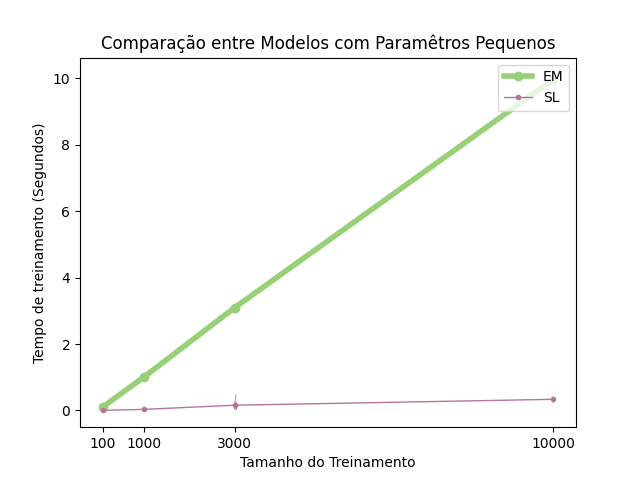
\includegraphics[width=\linewidth]{Figures/resultados/small_time}
        \caption{Tempo de treinamento para modelos pequenos}
    \end{subfigure}
    \hfill
    \begin{subfigure}[b]{0.3\linewidth}
        \centering
        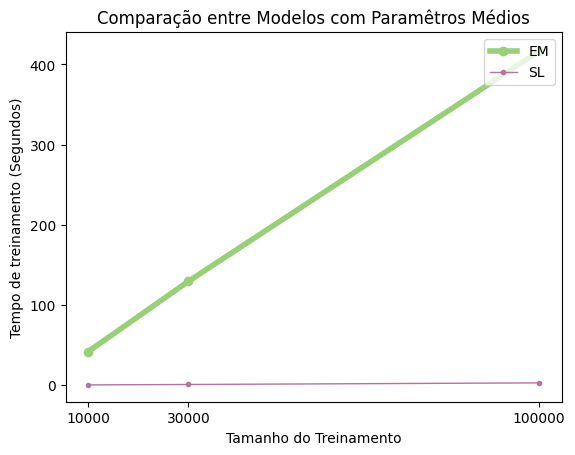
\includegraphics[width=\linewidth]{Figures/resultados/medium_time}
        \caption{Tempo de treinamento para modelos médios}
    \end{subfigure}
    \hfill
    \begin{subfigure}[b]{0.3\linewidth}
        \centering
        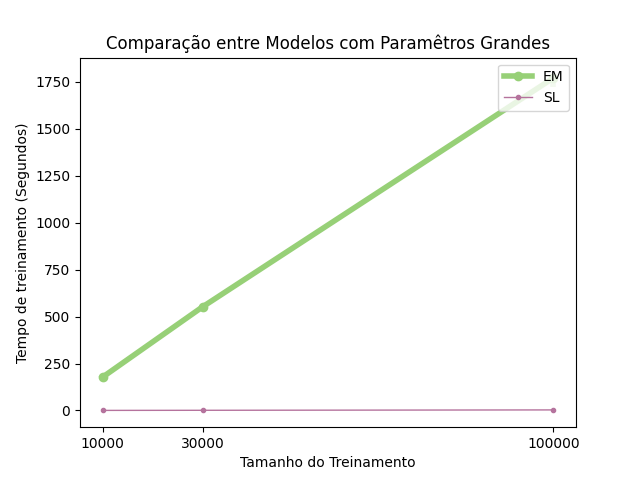
\includegraphics[width=\linewidth]{Figures/resultados/large_time}
        \caption{Tempo de treinamento para modelos grandes}
    \end{subfigure}
       \caption{Tempo a medida que o tamanho do treinamento aumenta }
       \label{fig:time}
\end{figure*}

\begin{figure*}
    \centering
    \begin{subfigure}[b]{0.3\linewidth}
        \centering
        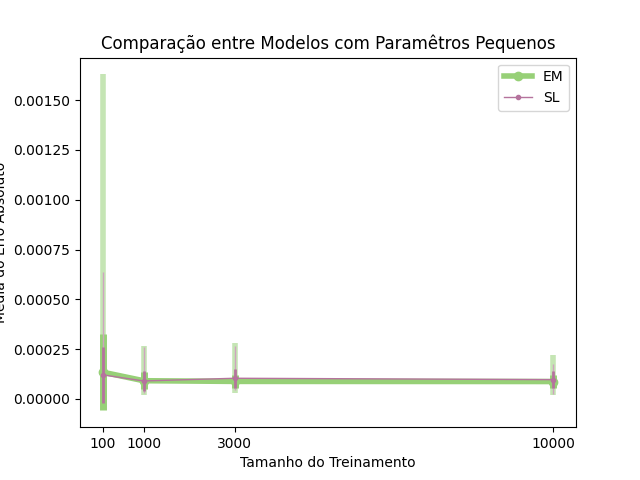
\includegraphics[width=\linewidth]{Figures/resultados/small_abs_prob_error}
        \caption{Erro médio absoluto para modelos pequenos}
    \end{subfigure}
    \hfill
    \begin{subfigure}[b]{0.3\linewidth}
        \centering
        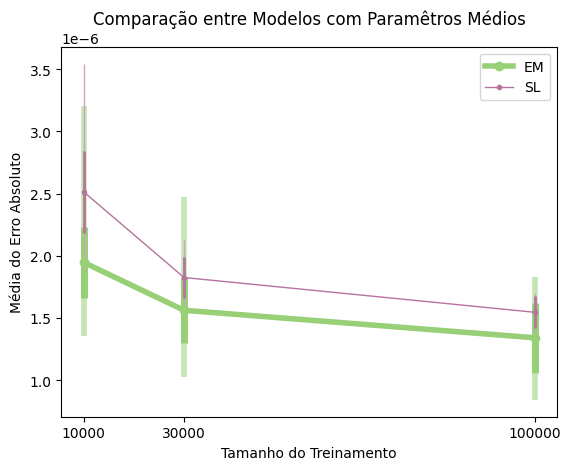
\includegraphics[width=\linewidth]{Figures/resultados/medium_abs_prob_error}
        \caption{Erro médio absoluto para modelos médios}
    \end{subfigure}
    \hfill
    \begin{subfigure}[b]{0.3\linewidth}
        \centering
        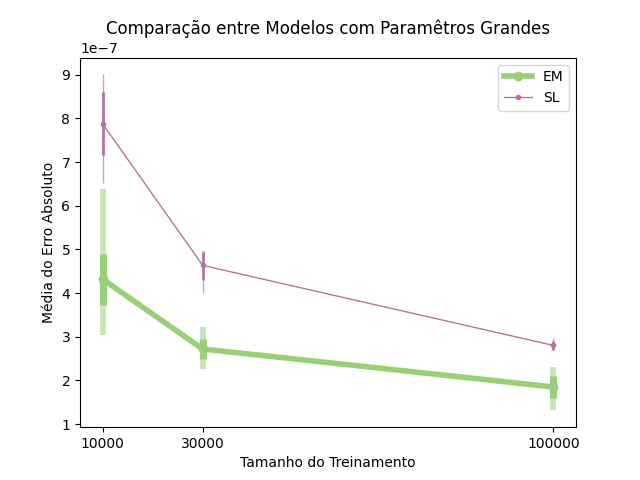
\includegraphics[width=\linewidth]{Figures/resultados/large_abs_prob_error}
        \caption{Erro médio absoluto para modelos grandes}
    \end{subfigure}
       \caption{Erro médio absoluto a medida que o tamanho do treinamento aumenta }
       \label{fig:abs_prob}
\end{figure*}

\begin{figure*}
    \centering
    \begin{subfigure}[b]{0.3\linewidth}
        \centering
        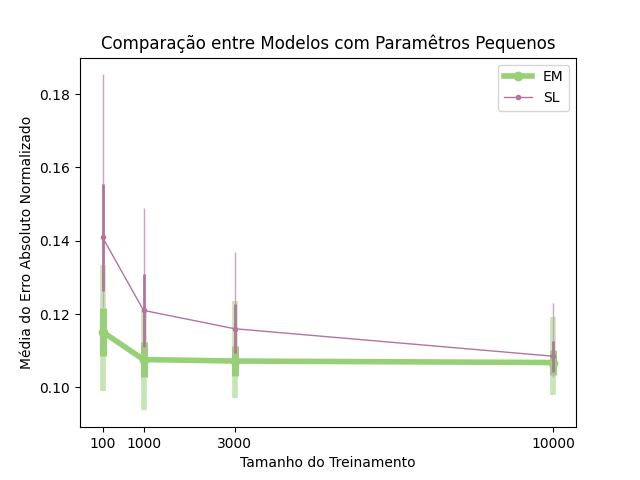
\includegraphics[width=\linewidth]{Figures/resultados/small_abs_norm_prob_error}
        \caption{Erro médio absoluto normalizado para modelos pequenos}
    \end{subfigure}
    \hfill
    \begin{subfigure}[b]{0.3\linewidth}
        \centering
        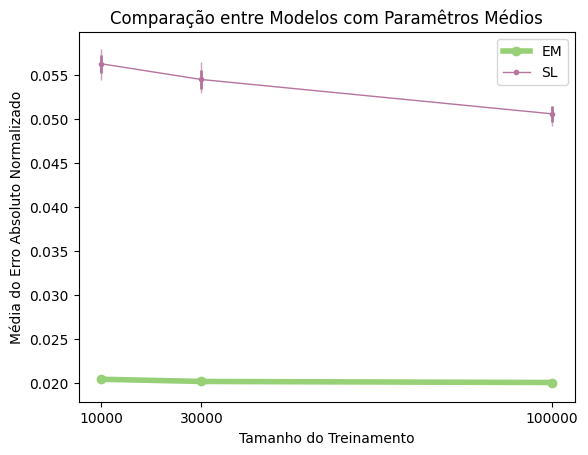
\includegraphics[width=\linewidth]{Figures/resultados/medium_abs_norm_prob_error}
        \caption{Erro médio absoluto normalizado para modelos médios}
    \end{subfigure}
    \hfill
    \begin{subfigure}[b]{0.3\linewidth}
        \centering
        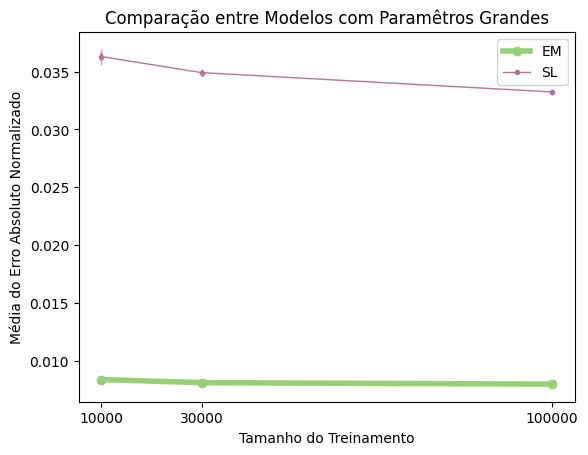
\includegraphics[width=\linewidth]{Figures/resultados/large_abs_norm_prob_error}
        \caption{Erro médio absoluto normalizado para modelos grandes}
    \end{subfigure}
       \caption{Erro médio absoluto normalizado a medida que o tamanho do treinamento aumenta }
       \label{fig:abs_norm_prob}
\end{figure*}

\begin{table*} 
    \caption{Configuração das sequências de comparações}
    \centering
    \begin{tabular}{l l l l}
        \toprule
        Tipo Modelo & Tamanho do Treinamento & Ambiente & Amostras \\
        \midrule
        Pequeno & 100, 1000, 3000, 10000 & Local / Nuvem & 15 $\times$ 15 \\
        Médio & 10000 & Local & 15 $\times$ 15 \\
        Médio & 10000, 30000 & Nuvem & 15 $\times$ 15 \\
        Médio & 100000 & Nuvem & 5 $\times$ 5 \\
        Grande & 10000 & Nuvem & 15 $\times$ 15 \\
        Grande & 30000, 100000 & Nuvem & 5 $\times$ 5 \\
        \bottomrule
    \end{tabular}
    \label{tab:config}
\end{table*}

Este experimento tem como o objetivo comparar a precisão e a velocidade de treinamento entre a implementação em Python de \textit{Spectral Learning} por H. Zhao, que será referenciado como \textit{SL}, e a implementação de um algoritmo de estimativa de \textit{Modelo Oculto de Markov} através do \textit{Método de Baum-Welch} também implementado em Python, que será referenciado como \textit{EM}.

\subsection{Metodologia}

\begin{figure}
    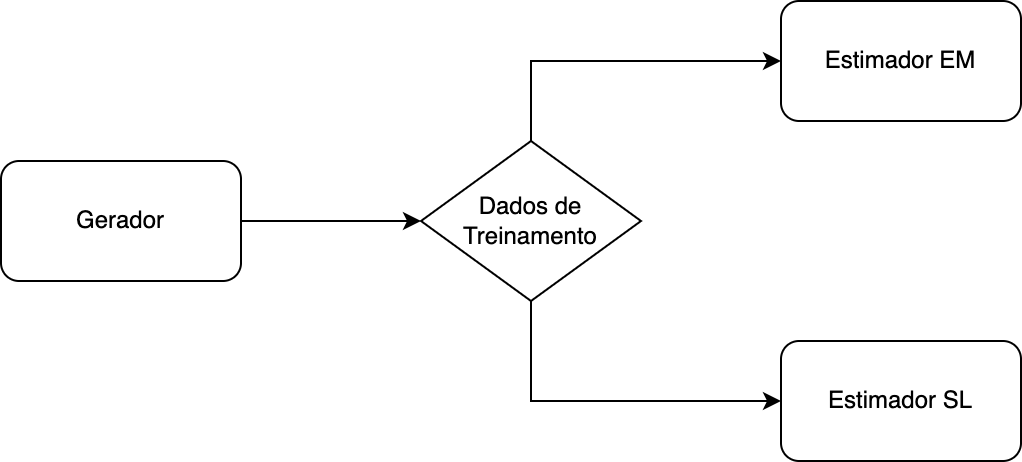
\includegraphics[width=\linewidth]{treinamento.png}
    \caption{Representação da configuração do treinamento dos modelos}
    \label{fig:trein}
\end{figure}

\begin{figure}
    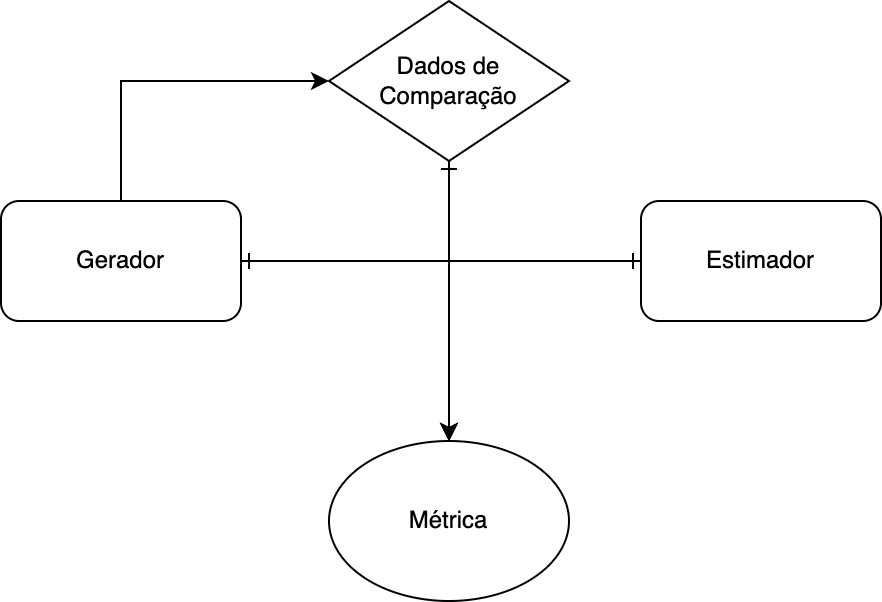
\includegraphics[width=\linewidth]{comparacao.png}
    \caption{Representação do passo de medida do erro dos modelos}
    \label{fig:comp}
\end{figure}

O experimento se inicia com o treinamento dos modelos como representado na figura \ref{fig:trein}. Para cada, modelo gerador, parametrizado por matrizes aleatórias, são geradas sequências de tamanho aleatório, entre $2$ e $30$ elementos, a serem utilizadas pelos modelos. Neste passo foi medido o tempo de treinamento dos modelos.

Num segundo momento, serão feitas as comparações entre as estimativas de probabilidade de cada modelo como representada na figura \ref{fig:comp}. Foram utilizadas duas formas de medir o erro, a média da diferença absoluta dos erros
\[
    Err_1 = \sum_{i=1}^n \frac{\vert P((o_i)_{i=1}^t) - \hat{P}((o_i)_{i=1}^t) \vert}{n}
\]
No qual $P$ é a probabilidade calculada pelo gerador e $\hat{P}$ é a probabilidade calculada pelo respectivo estimador.

A segunda forma de calcular o erro é dada por
\[
    Err_2 = \sum_{i=1}^n \frac{\vert P((o_i)_{i=1}^t) - \hat{P}((o_i)_{i=1}^t) \vert^{1/t}}{n}
\]
Nesta forma, que será chamada de média da diferença absoluta normalizada dos erros, deste modo erros em cadeias maiores são mais penalizados.

Foram treinados modelos de 3 tipos diferentes:
\begin{itemize}
    \item Pequenos: 4 estados ocultos, 8 símbolos observáveis;
    \item Médio: 20 estados ocultos, 40 símbolos observáveis;
    \item Grande: 50 estados ocultos, 100 símbolos observáveis
\end{itemize}

Por força da contingência de tempo, alguns experimentos foram feitos localmente se utilizando de um \textit{MacBook Pro mid 2014} equipado com um processador \textit{2,6 GHz Intel Core i5 Dual-Core}, em outros momentos utilizando uma \textit{instância EC2} da \textit{Amazon WebServices} do tipo \textit{C5}. A fornecedora não é capaz de dar precisão sobre a configuração da máquina, mas a instância utiliza pelo menos um \textit{Intel Xeon Platinum série 8000 de 1.ª geração}\autocite{AWS:2023EC2}. A tabela \ref{tab:config} apresenta a relação entre tipos de modelos, tamanhos dos treinamentos com seus respectivos ambientes de execução bem com a quantidade de vezes que os treinamentos foram repetidos, por exemplo, $15 \times 15$ significa que os modelos forem treinados contra $15$ geradores diferentes e no caso do estimador \textit{EM}, será feito $15$ vezes. Não faria sentido fazer mesmo com o estimador \textit{SL} porque para o mesmo conjuntos de sequências o resultado é o mesmo.

Todas as medidas de tempo foram feitas com os computadores de nuvem, que não correm o risco de ter interferências de outros processos que venham a comprometer a medida de tempo.

\subsection{Resultados}

Como consta na figura \ref{fig:time}, existe um grande contraste entre o custo de treinamento de estimadores \textit{EM} e \textit{SL}. Aquele é muito mais sensível ao aumento da quantidade de sequências.

Já no erro médio absoluto, o estimador \textit{SL} apresenta desvantagem. Apesar de ser bem sucedido em aprender modelos pequenos, ou pelo menos, aproximadamente, tão bem sucedido quanto \textit{EM}, na figura \ref{fig:abs_prob} para modelos maiores, os estimadores \textit{SL} começam em desvantagem, mas se aproximam do erro dos estimadores \textit{EM} a medida que o tamanho dos dados de treinamento aumentam. Apesar desta perspectiva otimista, as coisas pioram para os estimadores \textit{SL} na figura \ref{fig:abs_norm_prob}.

Como já discutido nas metodologias, o erro médio absoluto normalizado compensa o tamanho da sequência ao medir o erro. Apesar de algumas amostras demonstrarem um tendência de redução da diferença entre os erros, a distância decresce muito lentamente. Parece que, esta técnica erra muito ao estimar a probabilidade de sequências maiores.

\end{document}
